\documentclass{beamer}

\graphicspath{ {../dolgozat/images/} }
\usepackage[export]{adjustbox}
\usepackage{python}
\newcommand\tab[1][1cm]{\hspace*{#1}}

\usepackage{listings}
\usepackage{color}

% Code colorature
\definecolor{paszt}{RGB}{252,252,252}
\definecolor{keret}{RGB}{220,220,220}
\lstset{
backgroundcolor=\color{paszt},
% showlines=true,
framexleftmargin=4mm,
framexrightmargin=4mm,
framextopmargin=2mm,
framexbottommargin=2mm,
frameround=tttt,
frame=trbl,
rulecolor=\color{keret}
}

\usetheme{Copenhagen}
\useinnertheme{rectangles}

% ---- Mongo theme ----
%\definecolor{light-background}{RGB}{210,250,170}
%\definecolor{dark-background}{RGB}{128,92,64}
%\usecolortheme[RGB={220,250,180}]{structure}

% ---- Vanilla theme ----
% \definecolor{light-background}{RGB}{250,250,190}
% \definecolor{dark-background}{RGB}{128,92,64}
% \usecolortheme[RGB={210, 210, 140}]{structure}

% ---- Blue theme ----
%\definecolor{light-background}{RGB}{200,220,240}
%\definecolor{dark-background}{RGB}{100,110,120}
%\usecolortheme[RGB={180, 200, 230}]{structure}

% ---- Green theme ----
\definecolor{light-background}{RGB}{229,237,204}
\definecolor{dark-background}{RGB}{156,163,140}
\usecolortheme[RGB={180, 210, 150}]{structure}

\setbeamercolor{palette primary}{fg=black, bg=light-background}
\setbeamercolor{palette quaternary}{fg=white,bg=dark-background}

\setbeamercolor{title}{fg=black}
\setbeamercolor{frametitle}{fg=black}

% Set font
\usefonttheme{structurebold}

\frenchspacing

% Language packages
\usepackage[utf8]{inputenc}
\usepackage[T1]{fontenc}
\usepackage[magyar]{babel}

% AMS
\usepackage{amssymb,amsmath}

% Graphic packages
\usepackage{graphicx}

% Syntax highlighting
% \usepackage{listings}

\usepackage{tikz}

%\begin{figure}[htb]
%\begin{center}
%	\includegraphics[scale=0.4]{ps_times.png}
%\end{center}
%\end{figure}

% ==============
\begin{document}
% ==============

\title[Kínai karakterek felismerése, konvolúciós ANN]{
{\Large Kínai karakterek felismerése konvolúciós neurális
hálók használatával}
}
\author[Szilvási Péter]{\Large Szilvási Péter}
\date{Miskolci Egyetem, 2019. január 18.}

% --------------------
% Title page
\frame{\titlepage}

% --------------------
\begin{frame}[fragile]
\frametitle{Kínai karakterek felépítése}

\includegraphics[scale=0.6, center]{vonasrend}

\end{frame}

% --------------------
\begin{frame}[fragile]
\frametitle{OCR}

\begin{itemize}
\item Dokumentumok digitalizálása
\item Feldolgozási szintek: [2]\\
	Alacsony szintű \tab Középső szintű \tab Magas szintű
\end{itemize}

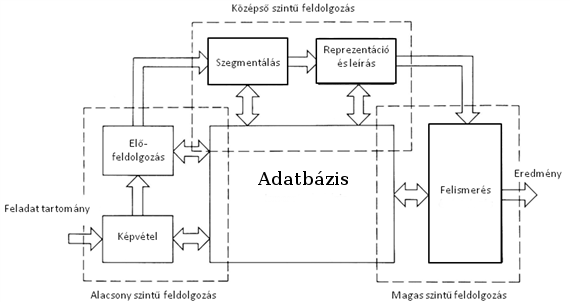
\includegraphics[scale=0.45, center]{ocr}

% Karakterek részekre bontása, struktúrális elemzése

% Betűtípusokból való eltérések

\end{frame}

% --------------------
\begin{frame}[fragile]
\frametitle{Jellemzők kinyerése, Dimenzió redukció}

\begin{itemize}
\item Főkomponens analízis (\textit{PCA})
	\begin{itemize}
		\item Magas dimenzió $\rightarrow$ Alsó dimenzió
		\item \(Av = \lambda v\)
	\end{itemize}
\item Kernelek alkalmazása
	\begin{itemize}
		\item Nem lineáris leképezések
	\end{itemize}
\item Neurális háló szerkezete\\
	\begin{center}
		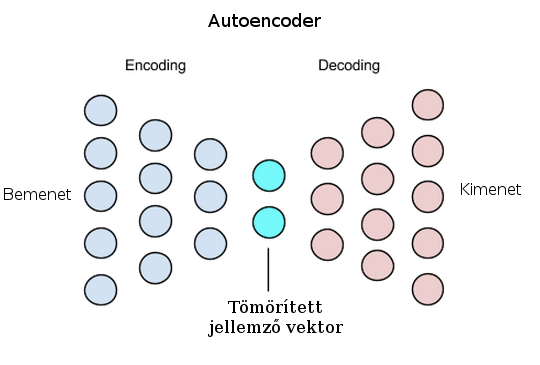
\includegraphics[scale=0.3]{deep_autoencoder}
	\end{center}
\end{itemize}

\end{frame}

% --------------------
\begin{frame}[fragile]
\frametitle{Mesterséges neurális hálók}

Neurális hálózatok [5]
\begin{itemize}
\item Rétegek
\item Elemei
\end{itemize}

Backpropagation
\begin{itemize}
\item Hiba $E_{total} = \sum \dfrac{1}{2}(target - output)^2.$
\item Láncszabály $\frac{\partial E_{total}}{\partial w_{5}} = \frac{\partial E_{total}}{\partial out_{o1}} \cdot \frac{\partial out_{o1}}{\partial net_{o1}} \cdot \frac{\partial net_{o1}}{\partial w_{5}}.$
\end{itemize}

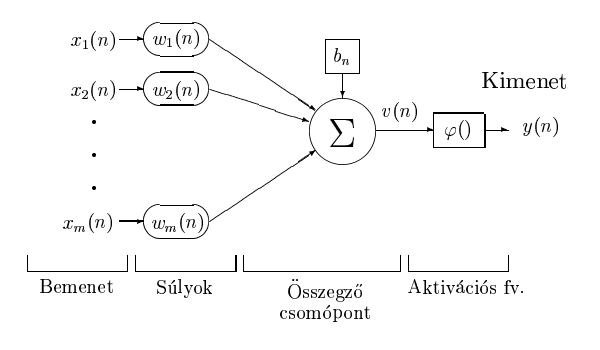
\includegraphics[scale=0.4, center]{ANNParts}

\end{frame}

% --------------------
\begin{frame}[fragile]
\frametitle{Konvolúciós neurális háló}
% A hálózat architektúrája, használt topológia
\begin{itemize}
\item Hálózat felépítése (konvolúciós rétegek $\rightarrow$ hagyományos ANN)
\item Bemenet $\rightarrow$ (\textit{Konvolúció $\rightarrow$ RELU $\rightarrow$ POOL}) $\rightarrow$ Kimenet(FC)
\end{itemize}
\begin{tabular}{c c}
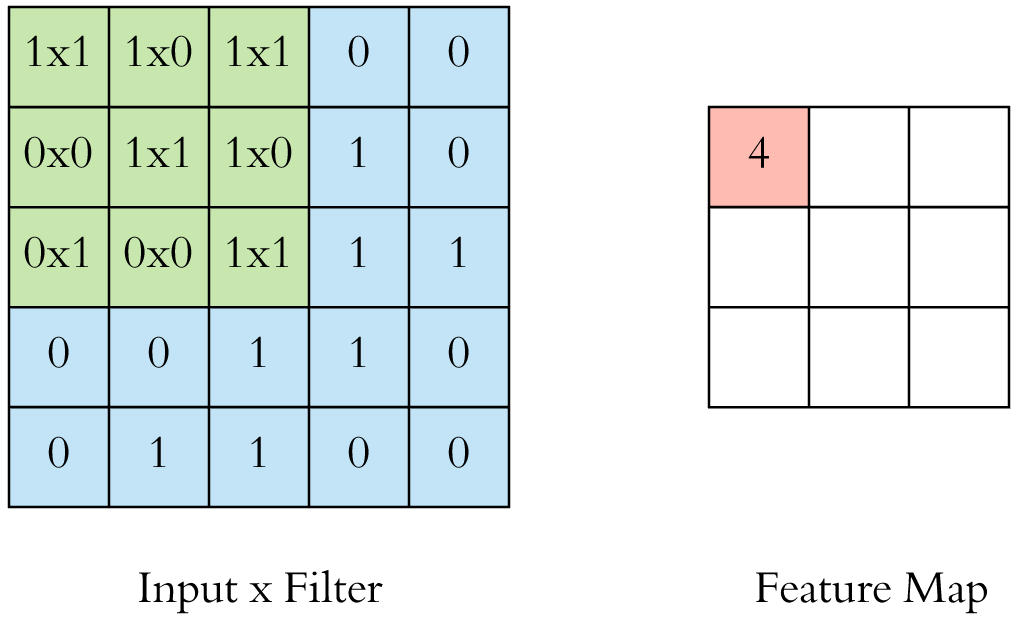
\includegraphics[scale=0.15]{convolution} & 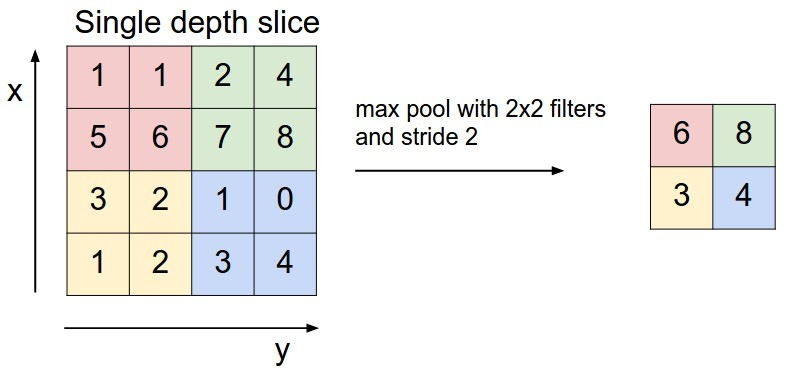
\includegraphics[scale=0.2]{maxpool}
\end{tabular}
\begin{itemize}
\item Hálózat tanítás
\end{itemize}
\begin{table}
\centering
\begin{tabular}{l l}
	1. Előre terjesztés & 3. Hiba visszaterjesztés\\
	2. Veszteség számítás & 4. Súly frissítés
\end{tabular}
\end{table}
\begin{itemize}
\item Dropout
\end{itemize}
\end{frame}

% --------------------
\begin{frame}[fragile]
\frametitle{Felismerés}

% 4.10-es ábra
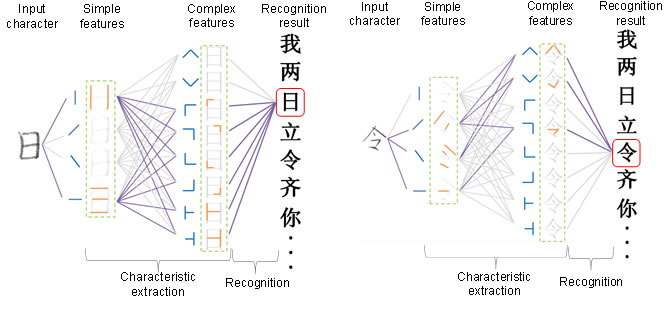
\includegraphics[scale=0.485]{CNN_CCR_working}

\end{frame}

% --------------------
\begin{frame}[fragile]
\frametitle{A hálózat architektúrája}

% 5.2 ábra
\begin{center}
	\includegraphics[scale=0.35]{NetworkArch}
\end{center}

\end{frame}


% --------------------
\begin{frame}[fragile]
\frametitle{Előfeldolgozás}

Adathalmaz: nyomtatott, kézzel írott, generált

\medskip

\includegraphics[scale=0.3, center]{input_images}

\begin{itemize}
\item Kép manipulálás:\\
Átméretezés \tab Forgatás \tab Zajosítás \tab Vágás\\
\begin{lstlisting} 
def resize():	def rotate():	def noise():
\end{lstlisting}
\item Konvertálás:\\
\begin{lstlisting}
for myFile in files:
    image = cv2.imread (myFile)
    train.append (image)
    train_labels.append([1., 0., 0., 0., 0.])
    
np.reshape() -> np.save()
\end{lstlisting}
\end{itemize}

\end{frame}

% --------------------
\begin{frame}[fragile]
\frametitle{Futtatás}
\begin{lstlisting}
time python3 train.py | tee log

Epoch 1/80
  12/2000 [............] loss:0.6964 acc: 0.7833
  24/2000 [............] loss:0.7951 acc: 0.7833
  36/2000 [............] loss:1.0486 acc: 0.7278
Epoch 80/80
  1992/2000 [========>.] loss:0.0385 acc:0.9871
  2000/2000 [==========] loss:0.0383 acc:0.9872
  
 real	19m40,397s
 user	55m4,422s
 sys	5m41,888s
\end{lstlisting}

\end{frame}

% --------------------
\begin{frame}[fragile]
\frametitle{Tesztelés}
\begin{itemize}
\item Kimenet létrehozés (.cvs) 
\item Model beolvasás
\begin{lstlisting}
model = load_model('model1.h5')
\end{lstlisting}
\item Kép átalakítás
\begin{lstlisting}
x = x.reshape((28,28,3))
\end{lstlisting}
\item Megjósolás
\begin{lstlisting}
x = model.predict(x)
\end{lstlisting}
\item Eredmény -> Kimeneti fájl
\end{itemize}
\end{frame}

% --------------------
\begin{frame}[fragile]
\frametitle{Hivatkozások}

% \begin{thebibliography}{9}

\begin{itemize}

\item[1] Tikk Domonkos: \textit{Optikai karakterfelismerés}, online melléklet, TypoTeX kiadó, 2006.

\smallskip

\item[2] Rövid A., Vámossy Z., Sergyán S.: \textit{A gépi látás és képfeldolgozás párhuzamos modelljei és algoritmusai}, 2014.

\smallskip

\item[3] Liu, Yin, Wang, Wang: \textit{Online and offline handwritten chinese character recognition: benchmarking on new databases}, Pattern Recognition, 2013.

\smallskip

\item[4] X. Wu, M. Wu: \textit{A recognition algorithm for chinese characters in diverse fonts}, Image Processing, 2002.

\smallskip

\item[5] Fazekas István: \textit{Neurális hálózatok}, Debreceni Egyetem, 2013.

\end{itemize}

% \end{thebibliography}

\end{frame}

% --------------------
\begin{frame}[fragile]
    \frametitle{\ }

\begin{center}
\Large \textbf{Köszönöm szépen a figyelmet!}
\end{center}

\end{frame}

\end{document}
